\documentclass[12pt,letterpaper]{article}

\usepackage{amsmath, amsthm}
\usepackage{graphicx,hyperref}
\usepackage{microtype, parskip}
\usepackage[numbers,sort&compress]{natbib}
\usepackage{lineno}
\usepackage{docmute}
\usepackage[font=small]{caption}
\usepackage{subcaption, multirow, morefloats}
\usepackage{wrapfig}
\usepackage{titlesec}
\usepackage{authblk, attrib, fullpage}
\usepackage{lineno}

\frenchspacing

\captionsetup[subfigure]{position = top, labelfont = bf, textfont = normalfont, singlelinecheck = off, justification = raggedright}

\begin{document}
\section{Results}

% posterior summary table
% latex table generated in R 3.1.2 by xtable 1.7-4 package
% Thu Jan  8 17:45:30 2015
\begin{table}[c]
  \centering
  \begin{tabular}{rrrrrrrrr}
    & mean & sd & 2.5\% & 25\% & 50\% & 75\% & 97.5\% & \(\hat{R}\) \\ 
    \hline
    alpha & 1.29 & 0.03 & 1.23 & 1.27 & 1.29 & 1.31 & 1.36 & 1.00 \\ 
    intercept & -0.78 & 0.14 & -1.05 & -0.87 & -0.78 & -0.68 & -0.51 & 1.00 \\ 
    logit(occupancy) & -0.53 & 0.08 & -0.69 & -0.59 & -0.53 & -0.48 & -0.38 & 1.00 \\ 
    log(size) & -0.05 & 0.05 & -0.14 & -0.08 & -0.05 & -0.01 & 0.05 & 1.00 \\ 
    ground dwelling & -0.28 & 0.10 & -0.47 & -0.34 & -0.28 & -0.21 & -0.09 & 1.00 \\ 
    scansorial & -0.22 & 0.11 & -0.43 & -0.29 & -0.22 & -0.14 & -0.00 & 1.00 \\ 
    herbivore & 0.09 & 0.09 & -0.09 & 0.03 & 0.09 & 0.14 & 0.27 & 1.00 \\ 
    insectivore & 0.10 & 0.11 & -0.11 & 0.03 & 0.10 & 0.17 & 0.31 & 1.00 \\ 
    omnivore & -0.12 & 0.11 & -0.33 & -0.19 & -0.12 & -0.05 & 0.09 & 1.00 \\ 
    \hline
    sd cohort & 0.33 & 0.06 & 0.23 & 0.29 & 0.33 & 0.37 & 0.48 & 1.00 \\ 
    sd phylogeny & 0.11 & 0.05 & 0.03 & 0.07 & 0.10 & 0.14 & 0.23 & 1.03 \\ 
    \hline
  \end{tabular}
  \caption{Marginal posterior estimates for the praameters of interested based on 1000 posterior samples. The intercept can be interpreted as the estimate for the mean observed species. The other values are the effect of a trait on the expected species duration as expressed as deviation from the mean. The categorical variables are binary index variables where an observation is of that category or not. \(\hat{R}\) values of less than 1.1 indicate approximate chain convergence for the posterior samples.}
  \label{tab:post_sum}
\end{table}




\begin{figure}[ht]
  \centering
  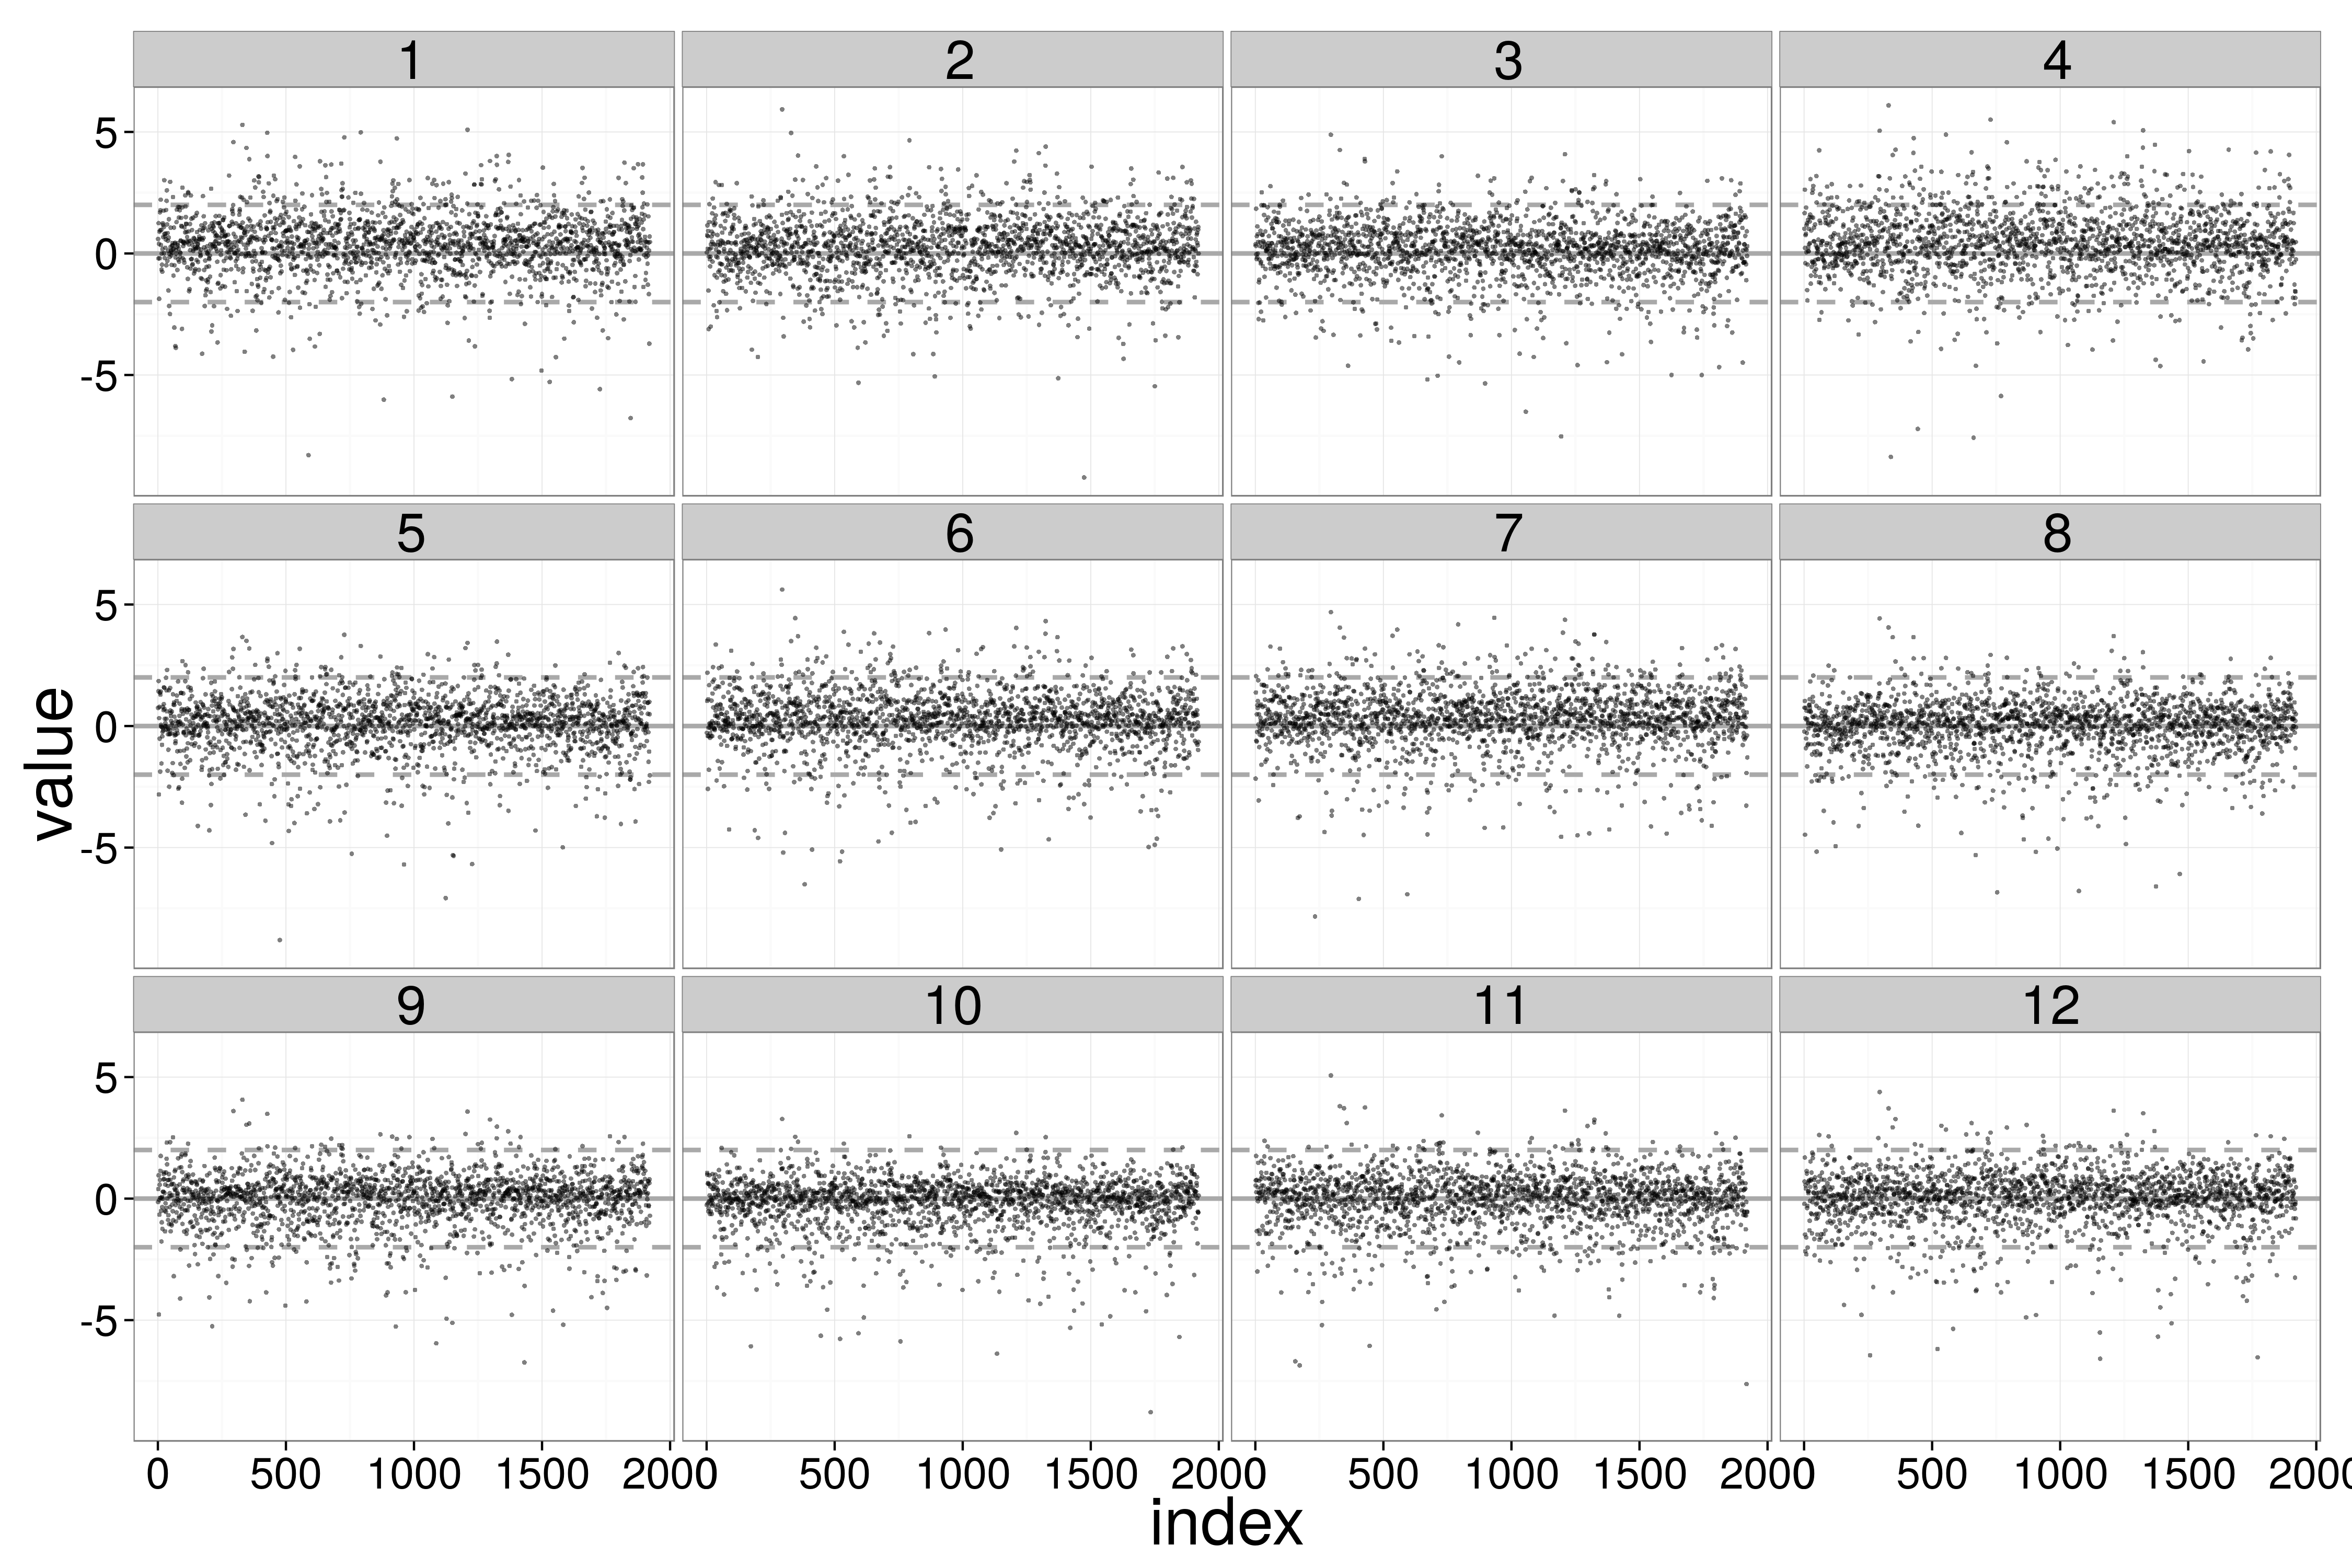
\includegraphics[height = 0.5\textheight, width = \textwidth, keepaspectratio = true]{figure/residual_plot}
  \caption{Deviance residuals from the fitted survival model. Each graph depicts the residuals from single draws from the posteriors distributions of all estimated parameters. Positive values indicate an under estimate of the observed duration, while negative values indicate an over estimate of the observed duration. Twelve difference examples are provided here to indicate the lack of individual observation based biases.}
  \label{fig:ppc_res}
\end{figure}

\begin{figure}[ht]
  \centering
  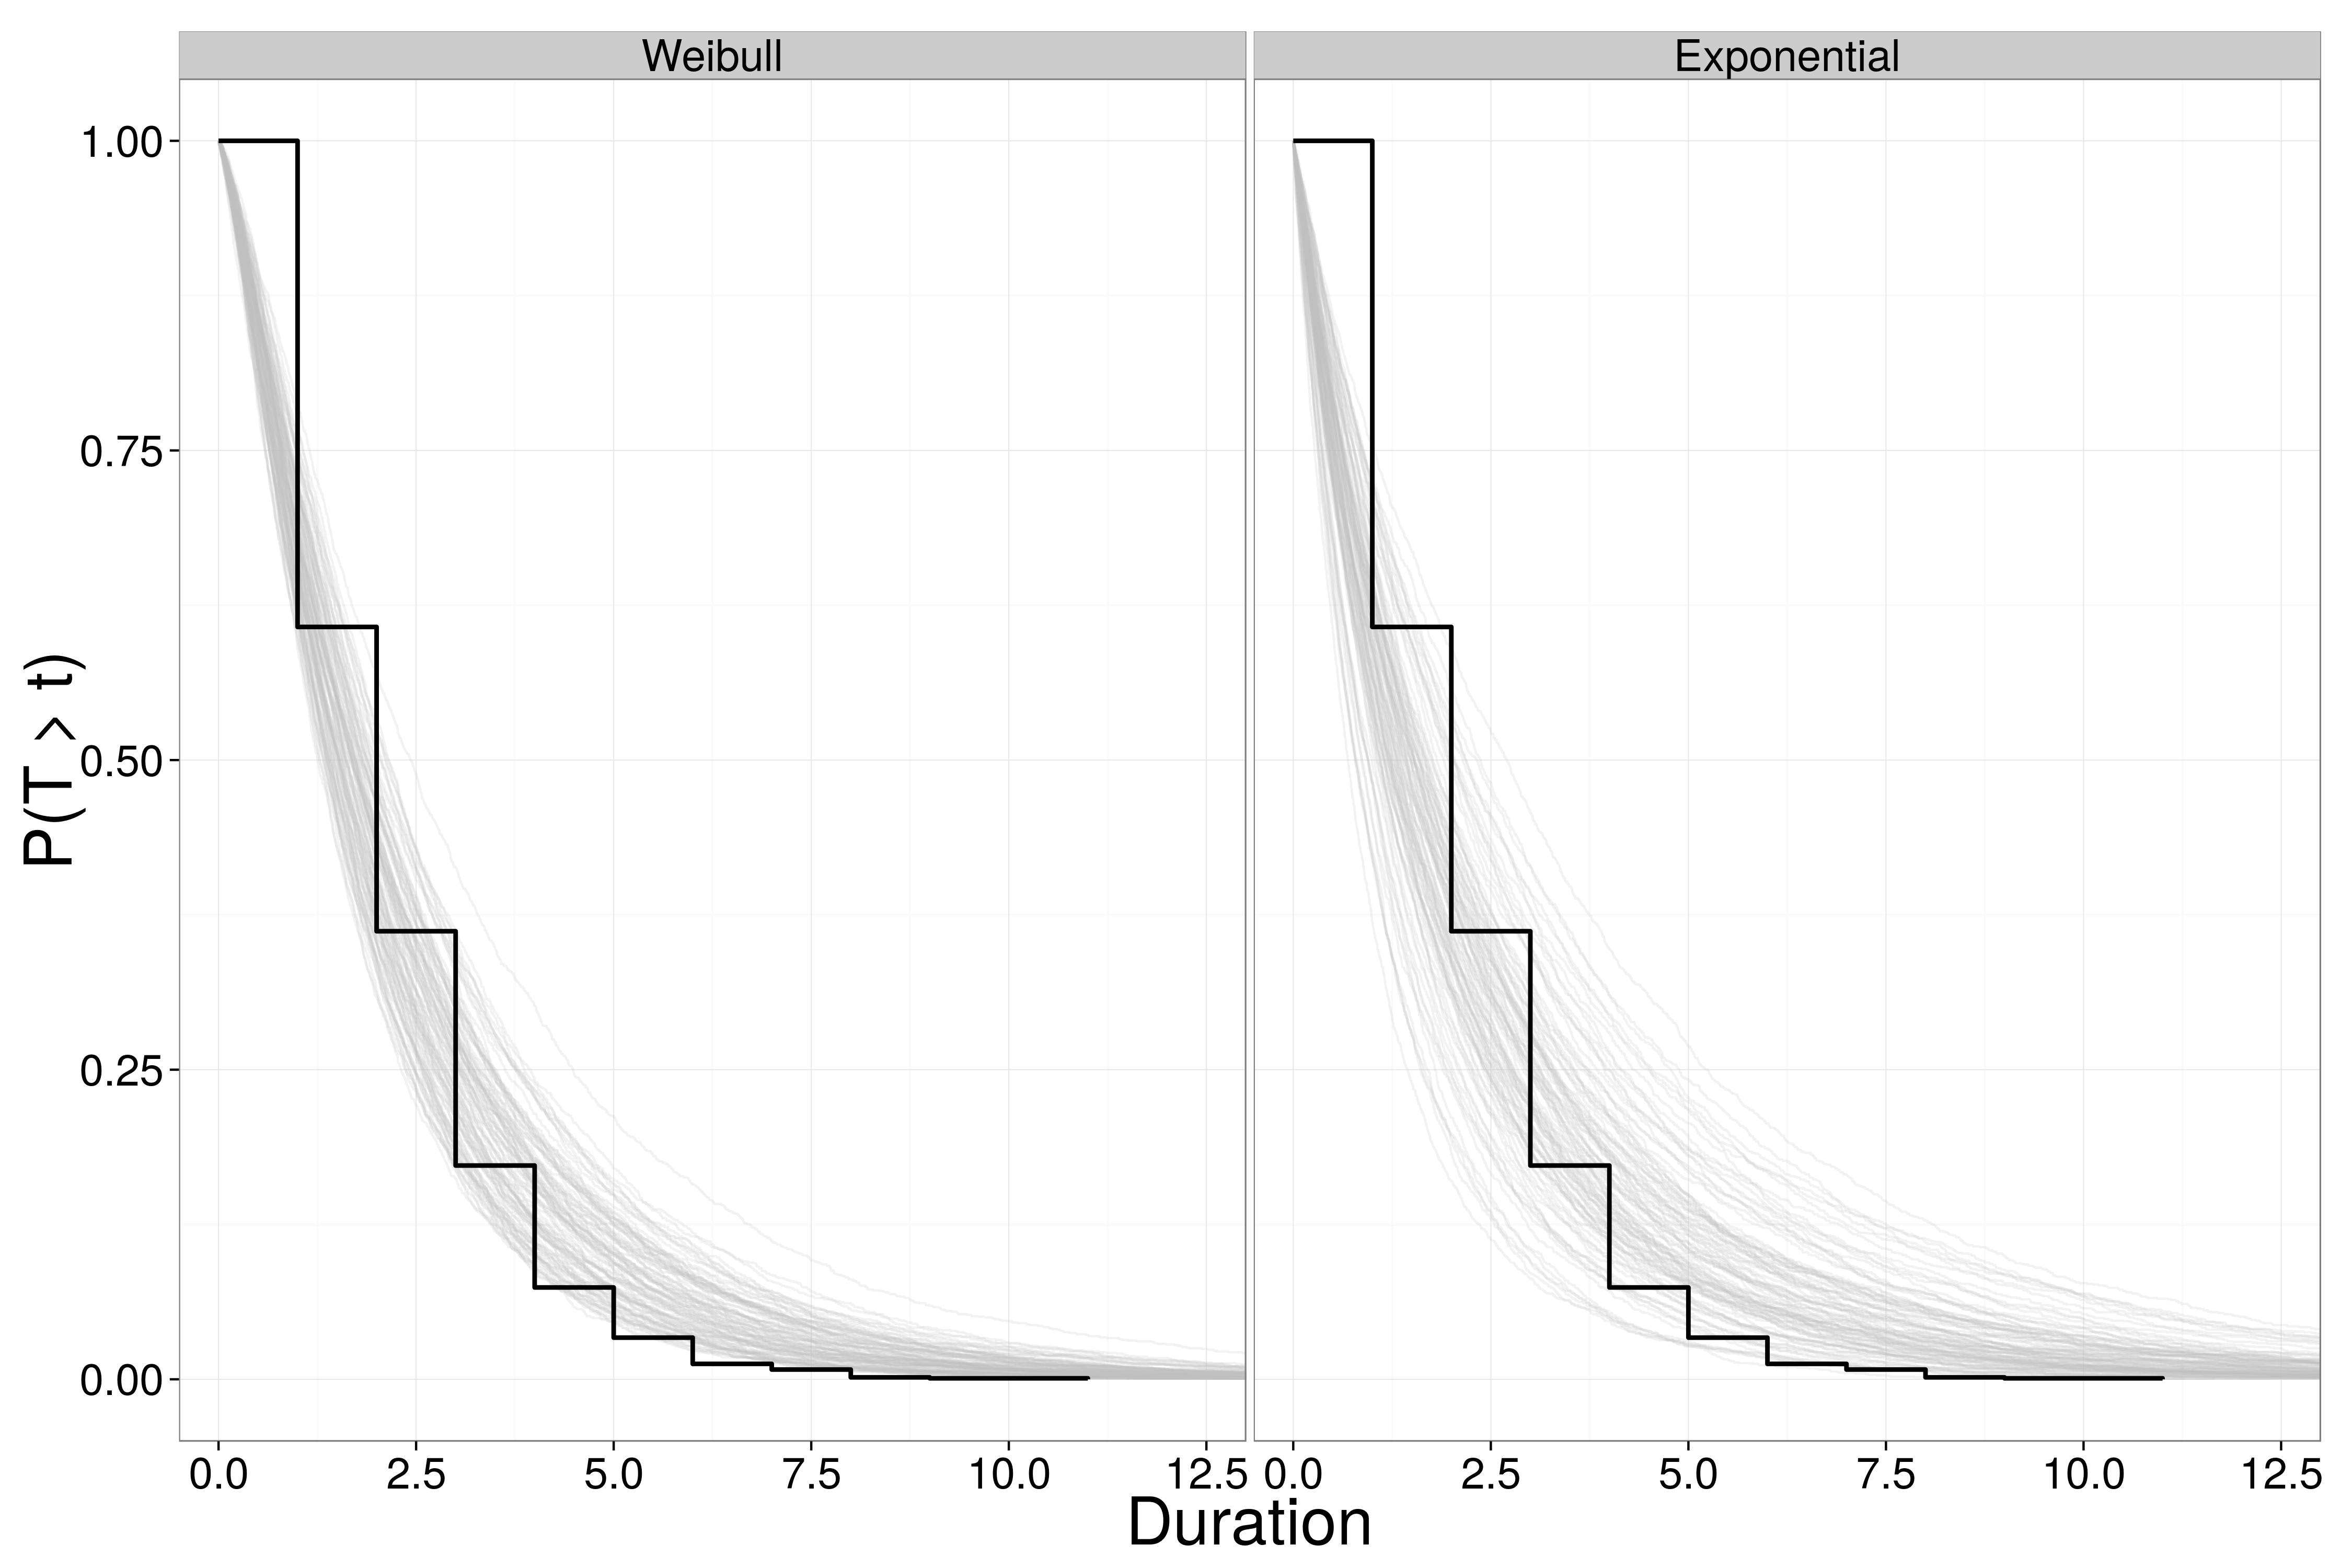
\includegraphics[height = 0.5\textheight, width = \textwidth, keepaspectratio = true]{figure/survival_function}
  \caption{Comparison between K-M estimate of survival function (black) from the observed versus K-M estimates from 100 simulated data sets using the fitted model (dark grey). Simulated data sets were generated by drawing parameter values randomly from their estimated posteriors and using the observed covariate information to estimate durations for all the observed species. On the left are the results from the full survival model (Fig. \ref{fig:model_diagram}), while on the right are the results from a simplified model where duration follows an exponential distribution and there is no phylogenetic effect.}
  \label{fig:ppc_surv}
\end{figure}

\begin{figure}[ht]
  \centering
  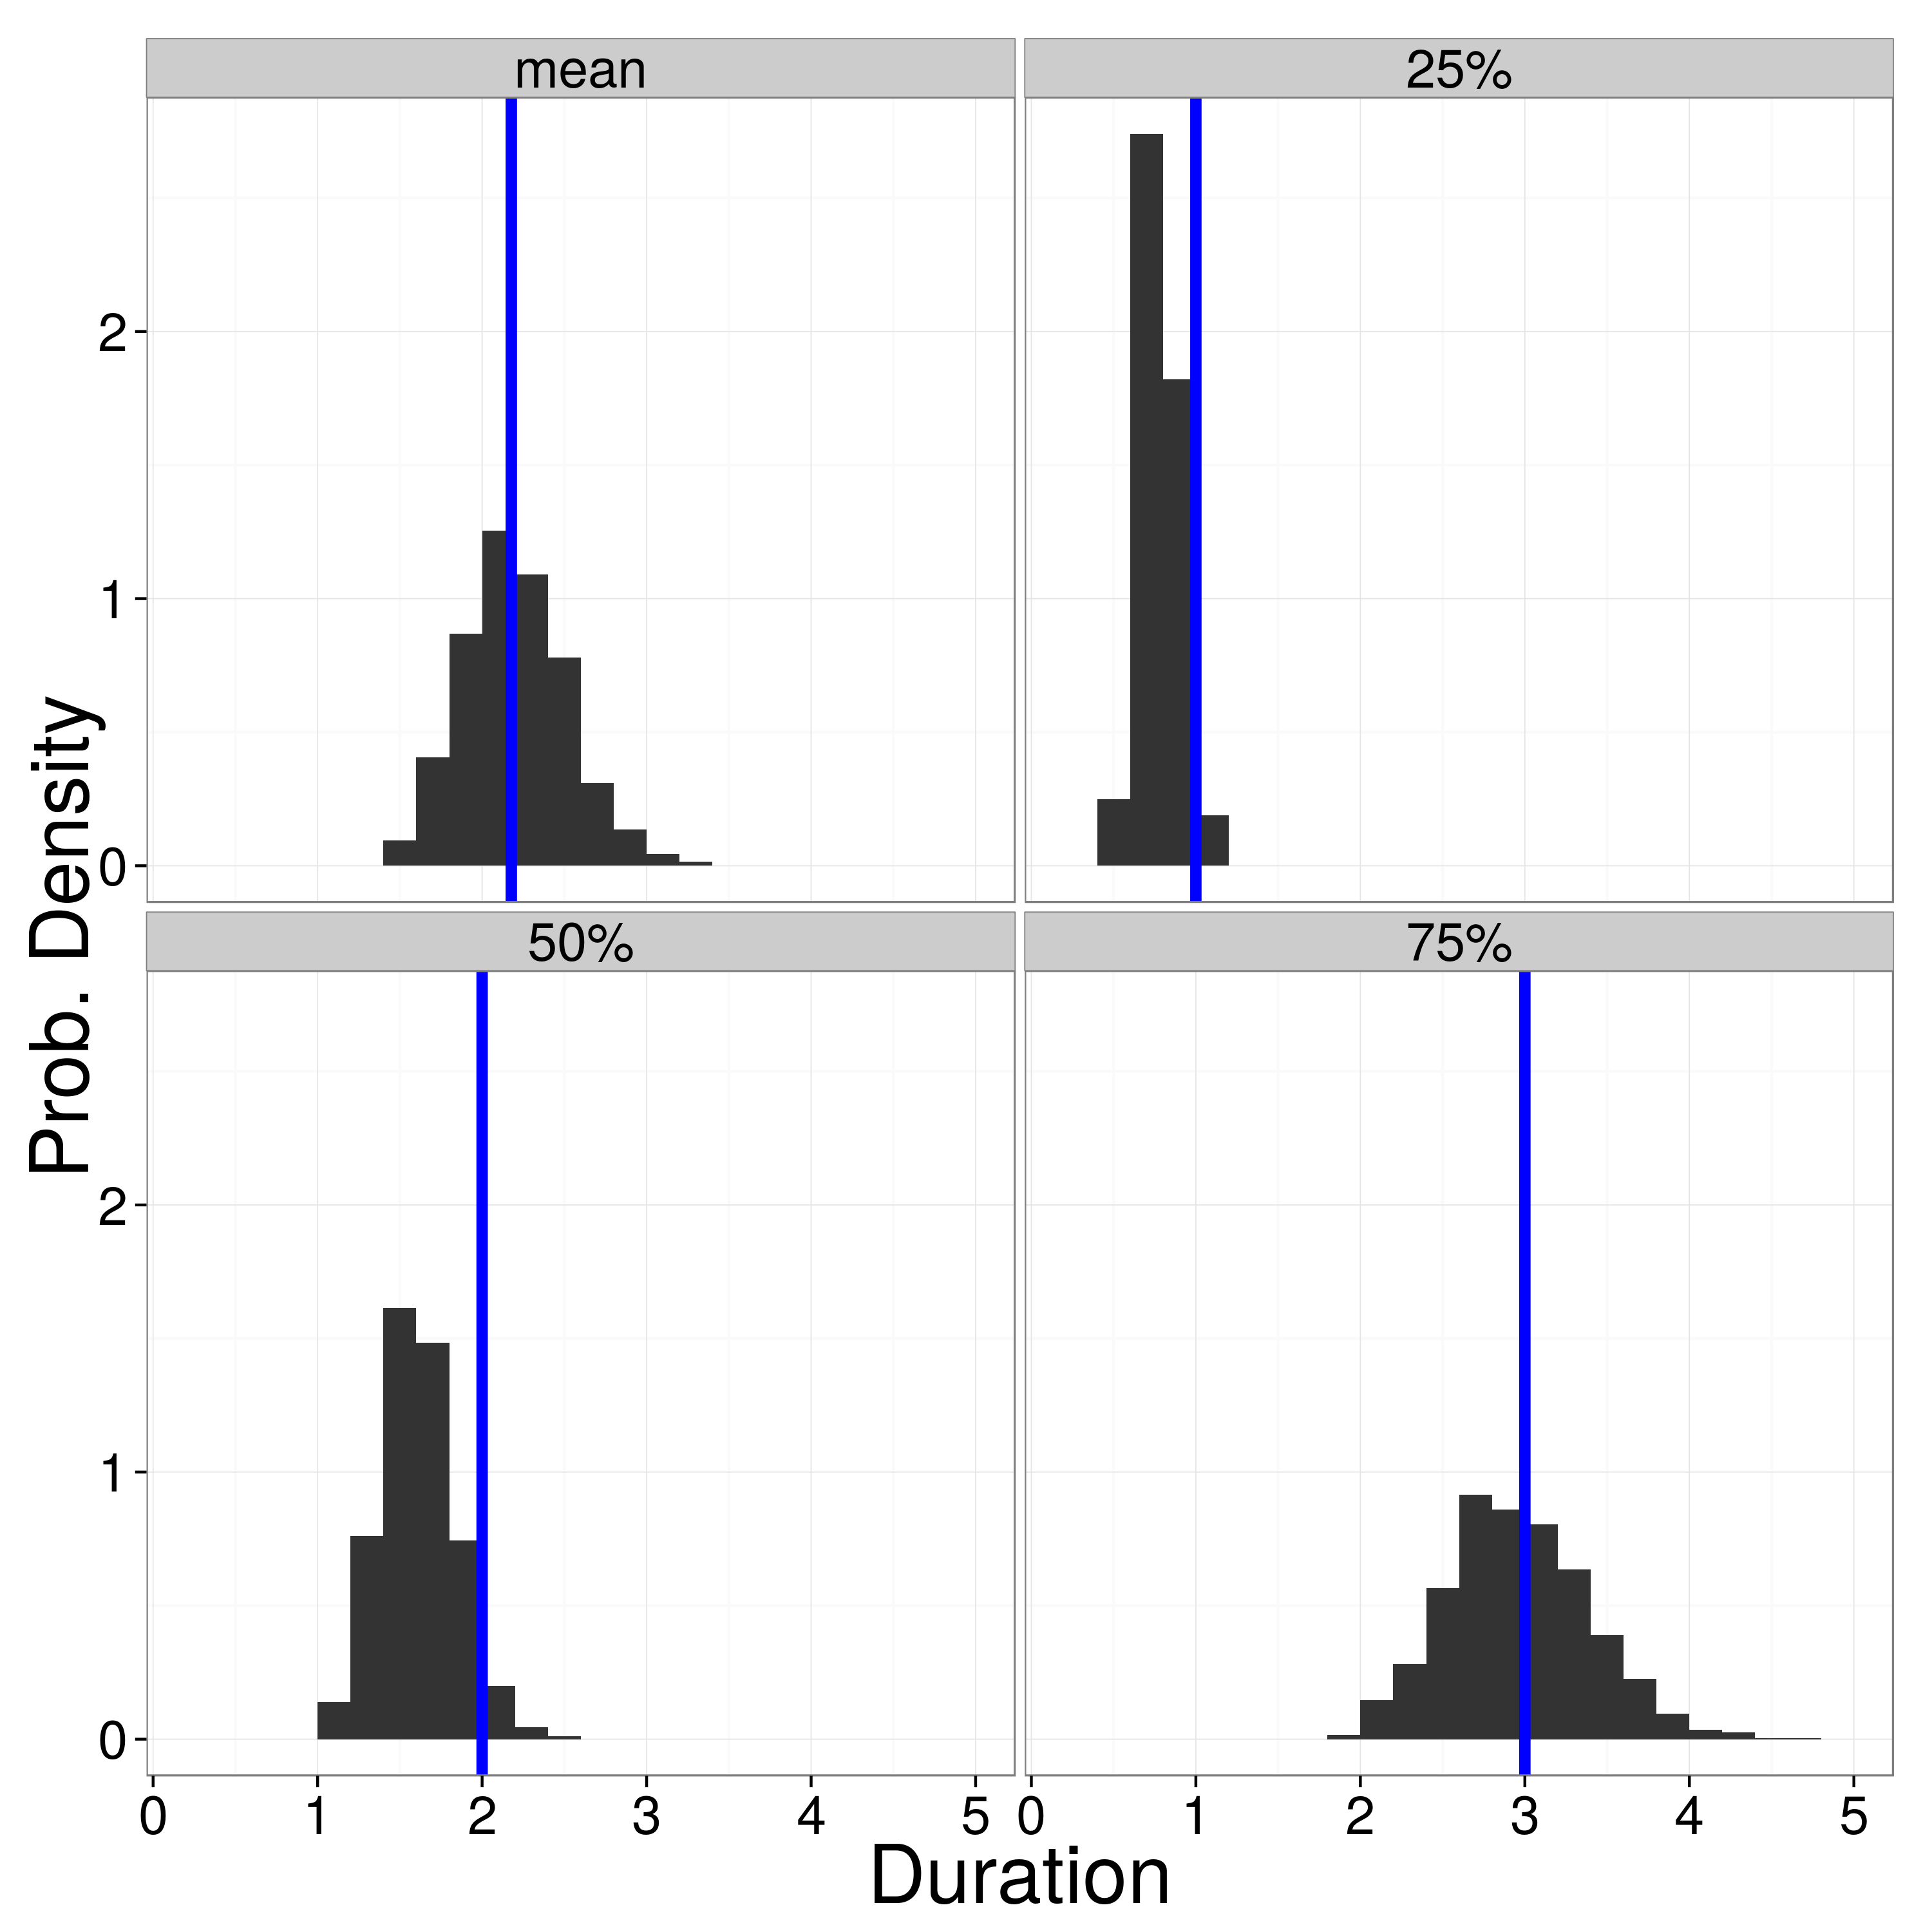
\includegraphics[height = 0.5\textheight, width = \textwidth, keepaspectratio = true]{figure/quant_ppc}
  \caption{The results of additional posterior predictive checks for four summaries of the observed durations, as labeled. Blue vertical indicate the observed value. None of the observed are significantly different from the posterior predictive distributions.}
  \label{fig:ppc_quant}
\end{figure}

\begin{figure}[ht]
  \centering
  \begin{subfigure}[b]{0.4\textwidth}
    \caption{}
    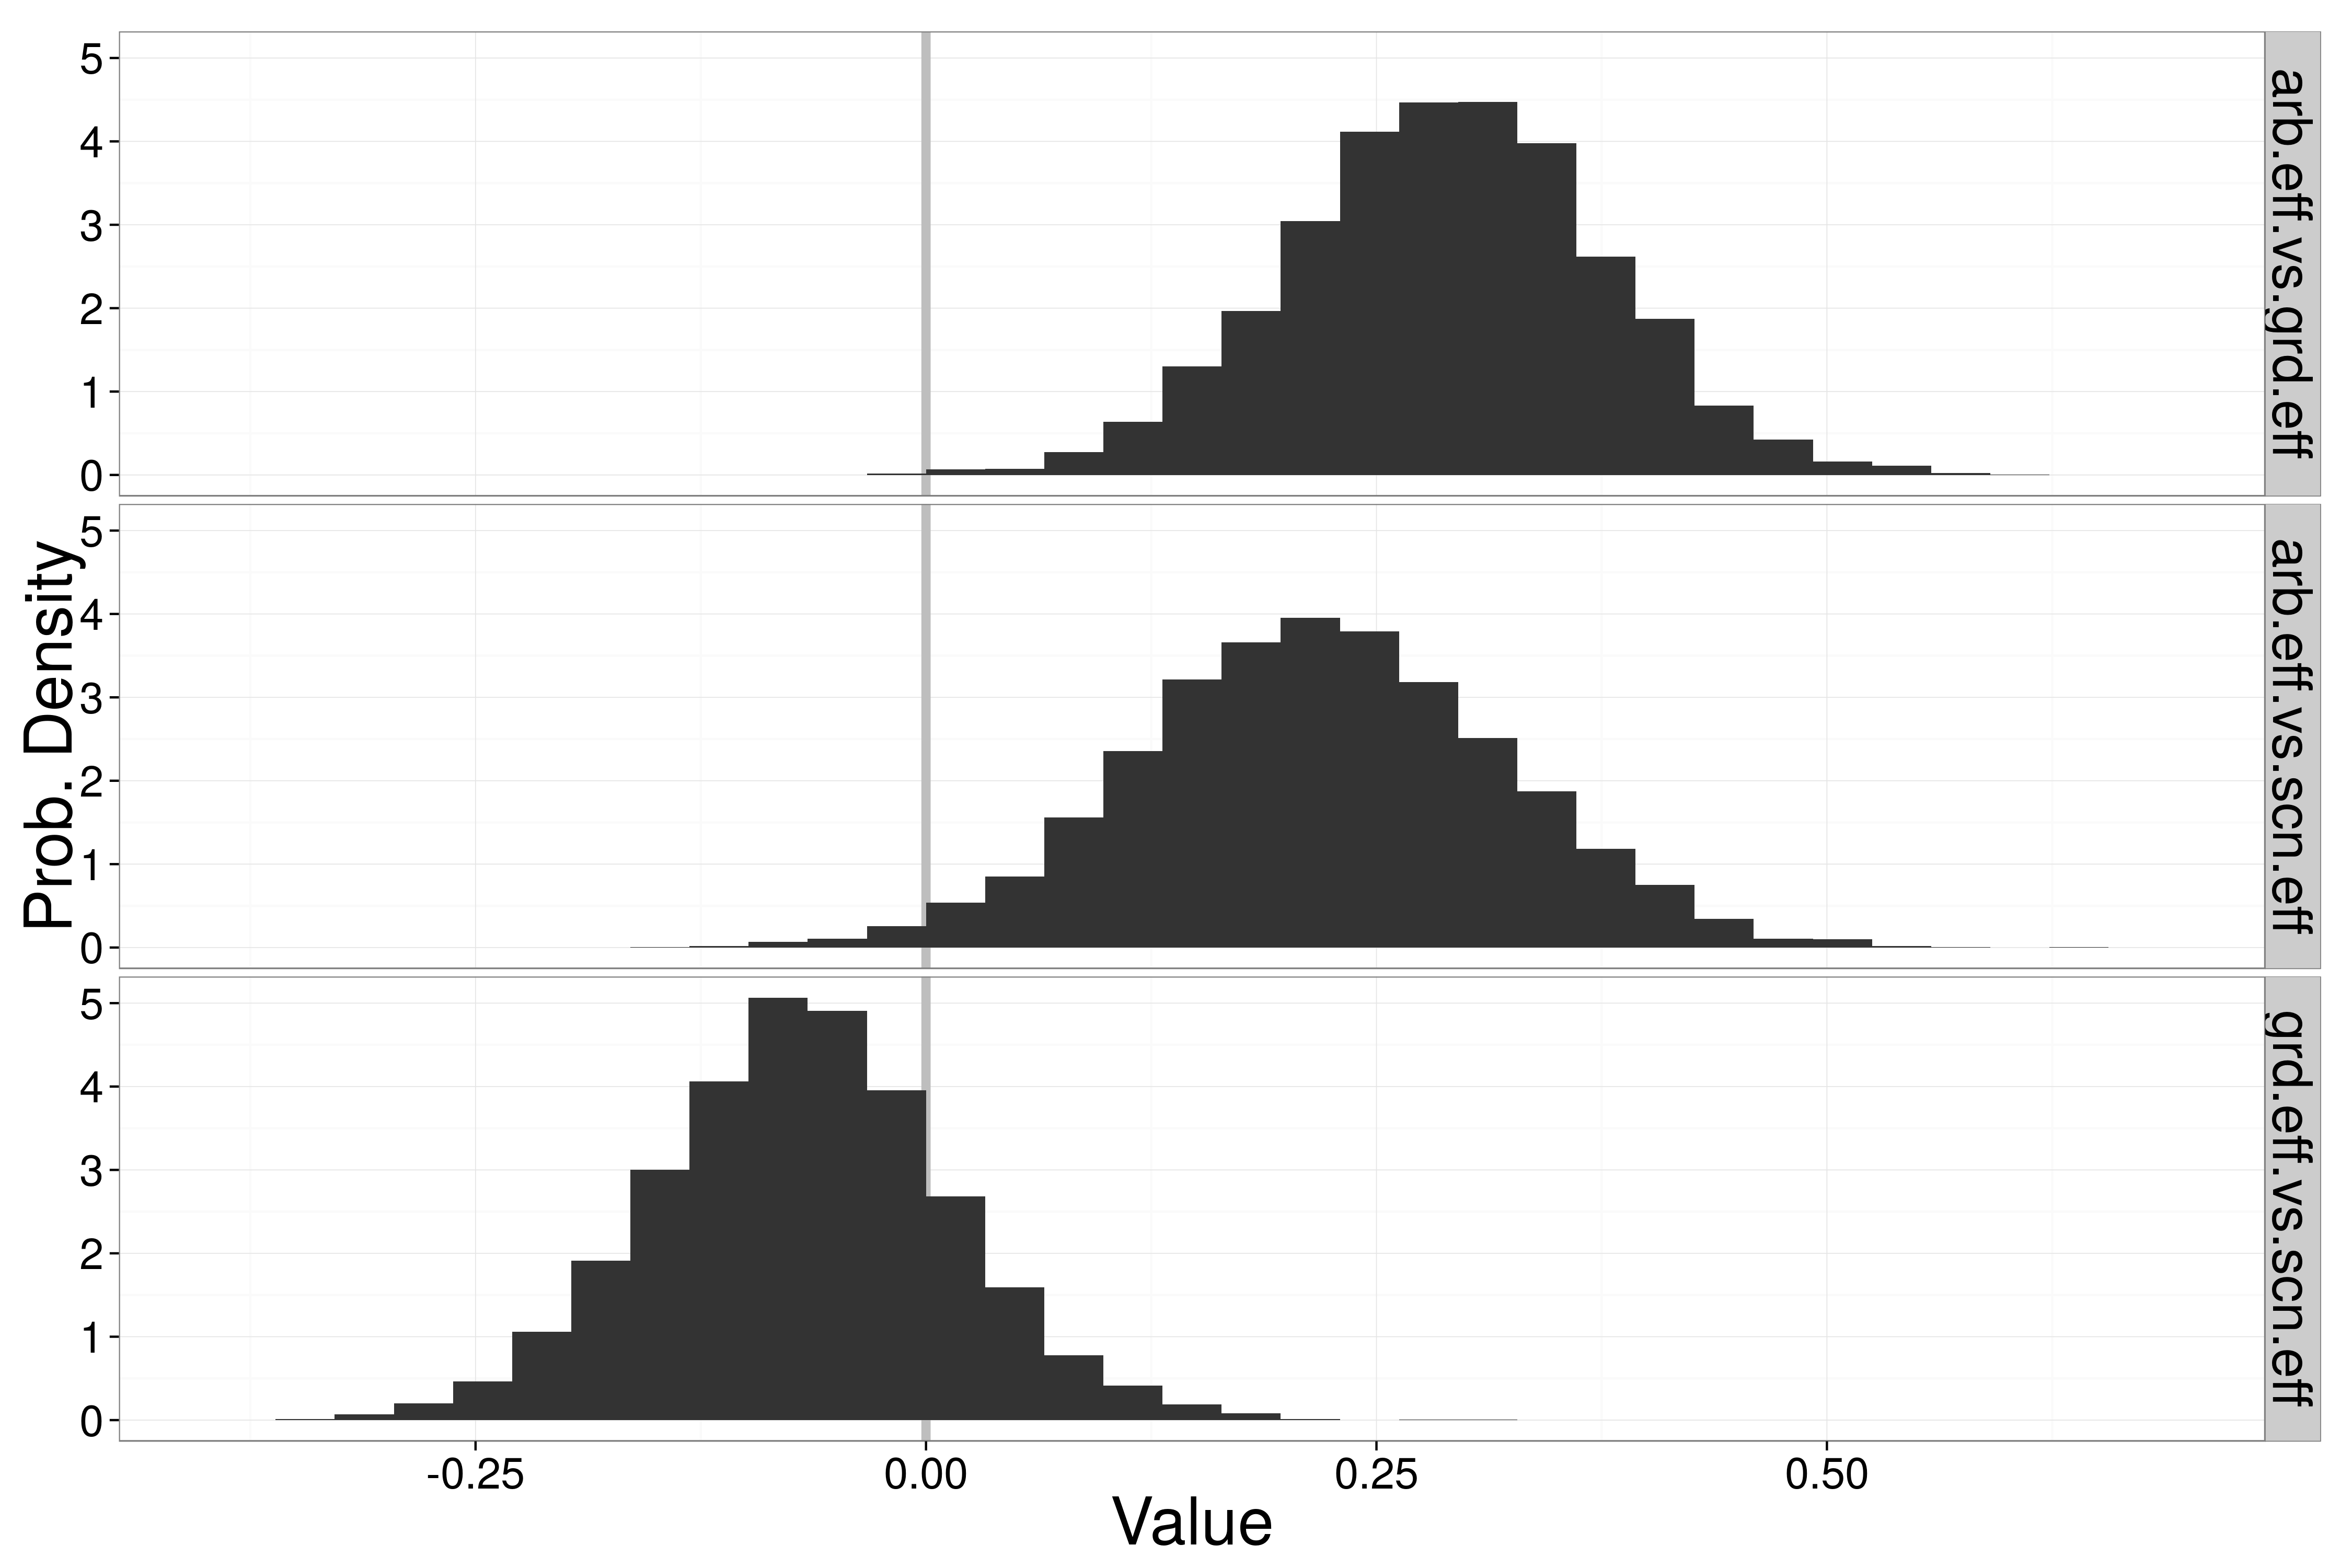
\includegraphics[height = 0.5\textheight, width = \textwidth, keepaspectratio = true]{figure/loco_diff_est}
    \label{subfig:loco}
  \end{subfigure}
  \begin{subfigure}[b]{0.4\textwidth}
    \caption{}
    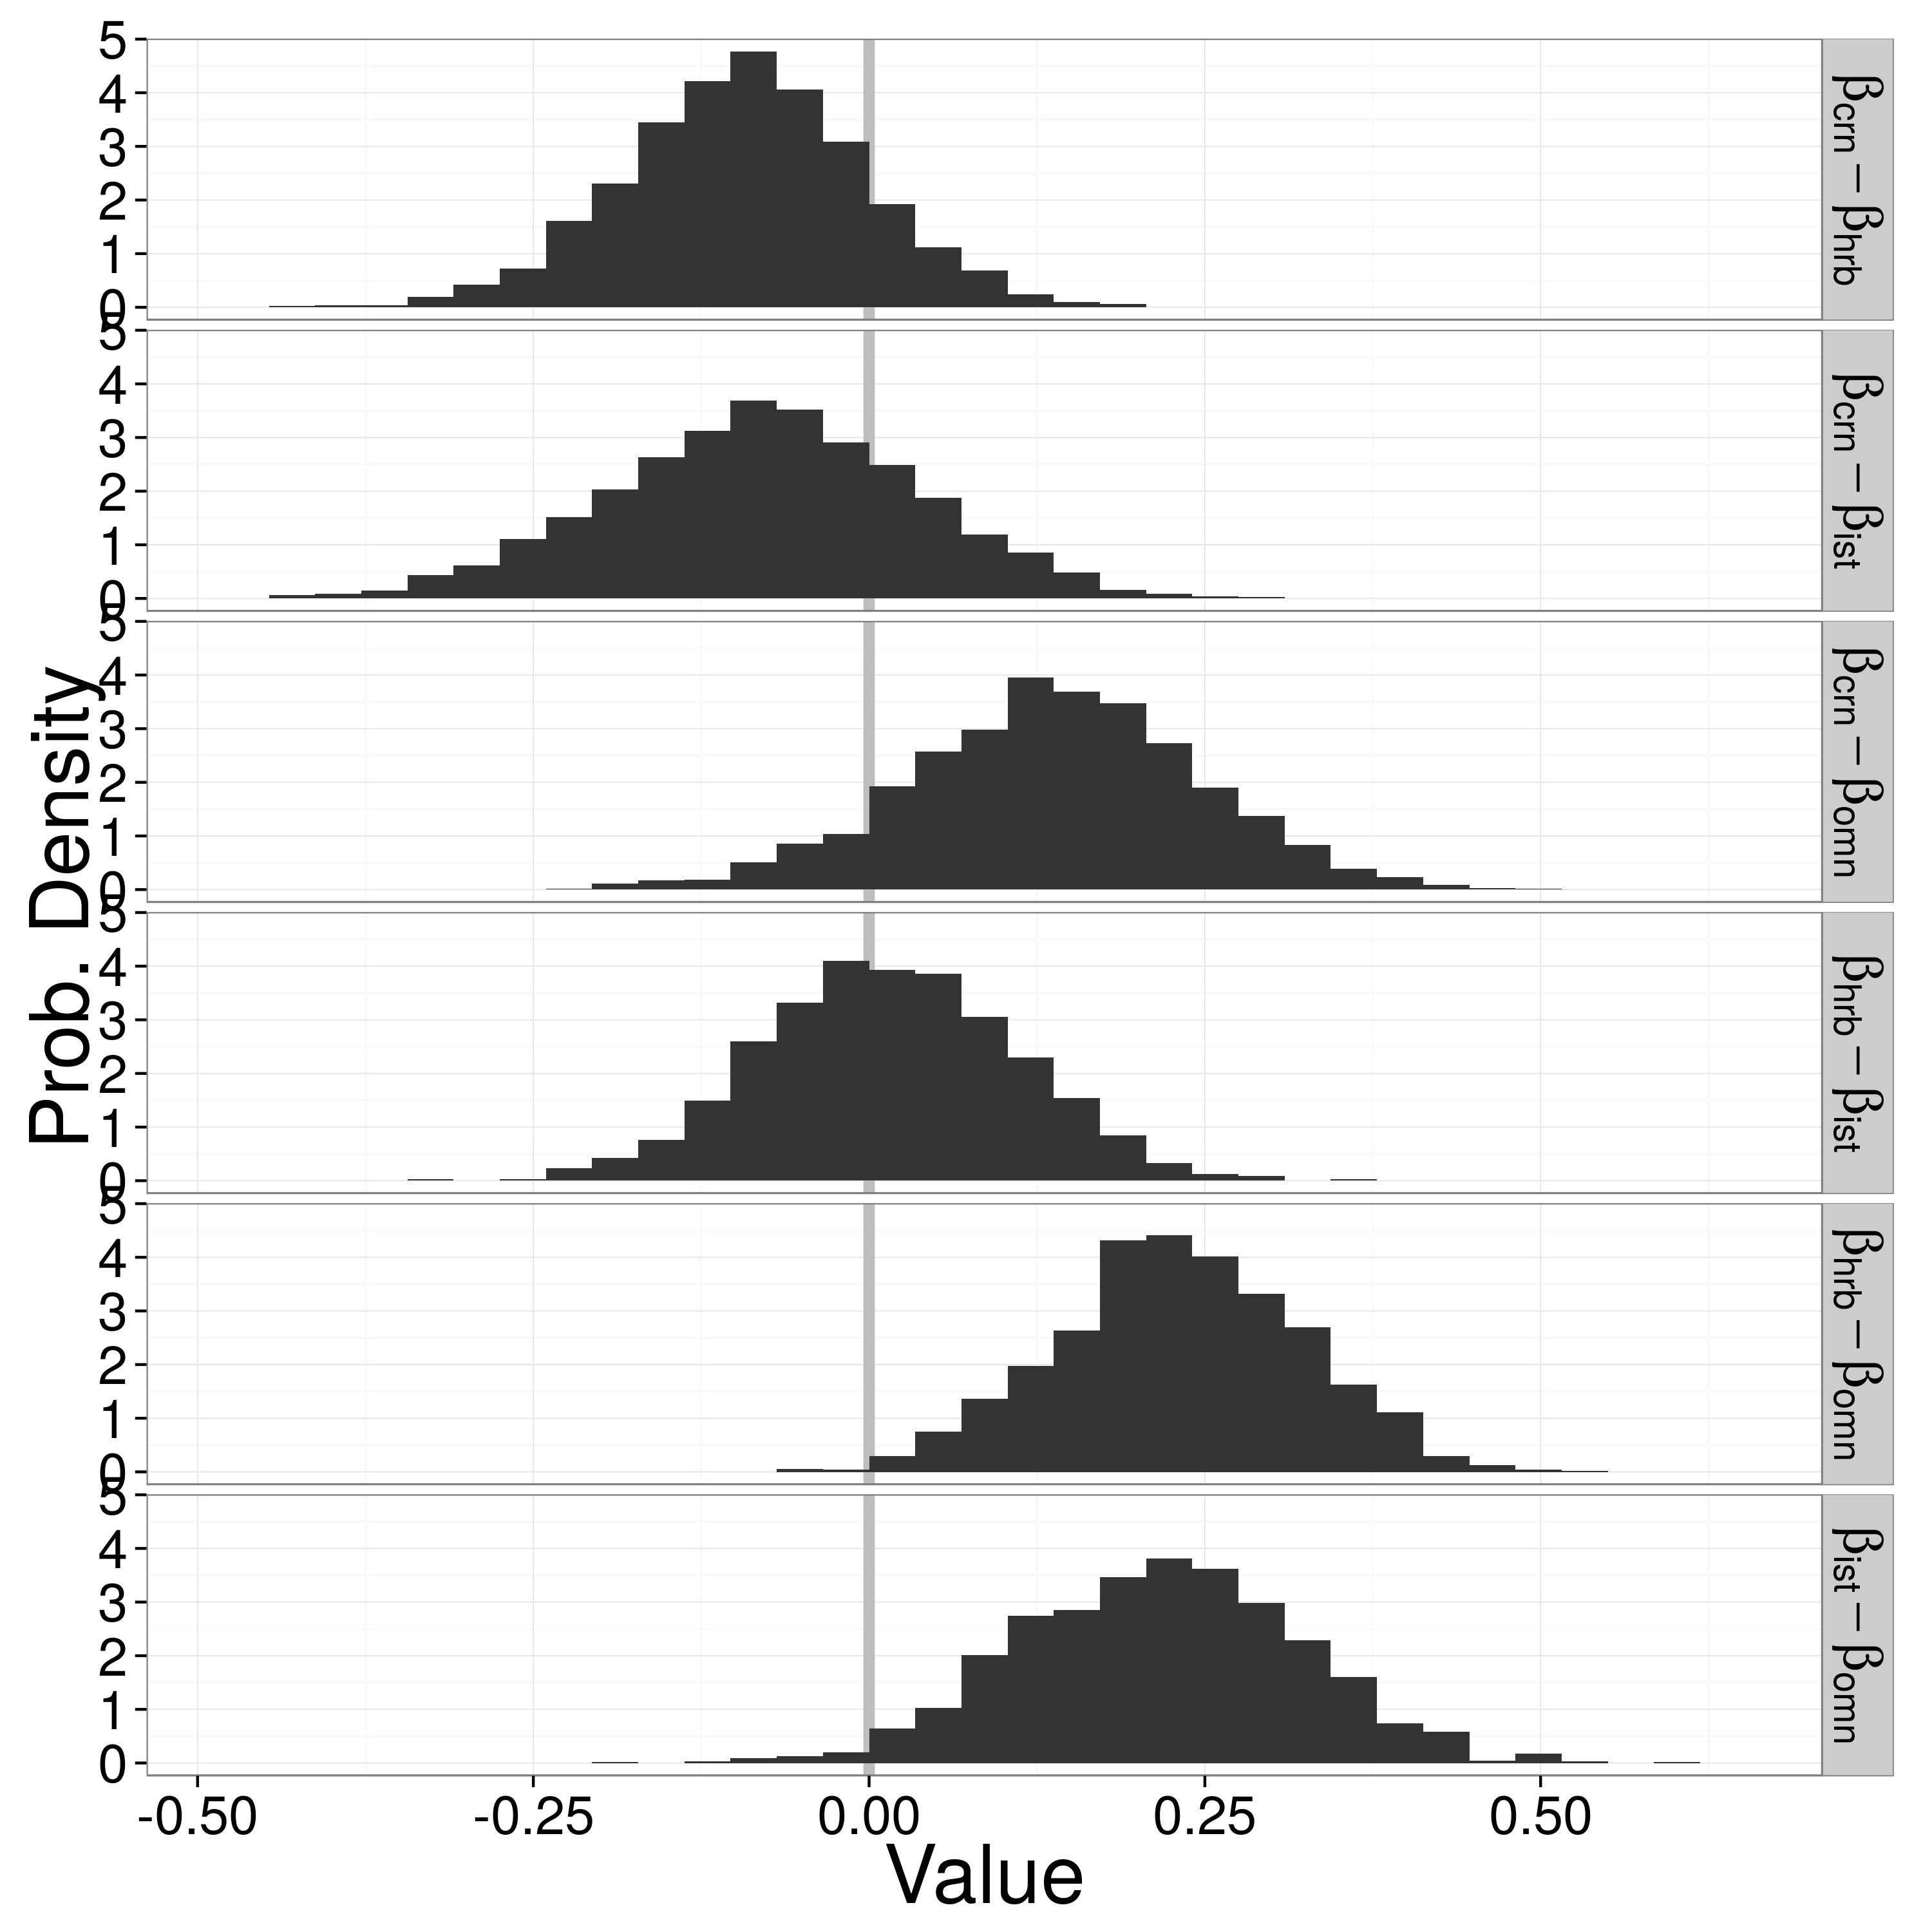
\includegraphics[height = 0.5\textheight, width = \textwidth, keepaspectratio = true]{figure/diet_diff_est}
    \label{subfig:diet}
  \end{subfigure}
  \caption{Pairwise differences in effect of the locomotor (\subref{subfig:loco}) and dietary categories (\subref{subfig:diet}) on expected duration from 1000 samples from the posterior distribution. Comparisons of locomotor categories, from top to bottom (\subref{subfig:loco}), are: arboreal versus ground dwelling, arboreal versus scansorial, and ground dwelling versus scansorial. For dietary category, from top to bottom (\subref{subfig:diet}): carnivore versus herbivore, carnivore versus insectivore, carnivore versus omnivore, herbivore versus insectivore, herbivore versus omnivore, and insectivore versus omnivore. Values to the left indicate that the first category is expected to have a greater duration than the second, while values to the right indicate that the first category is expected to have a shorter duration.}
  \label{fig:loco_est}
\end{figure}


\begin{figure}[ht]
  \centering
  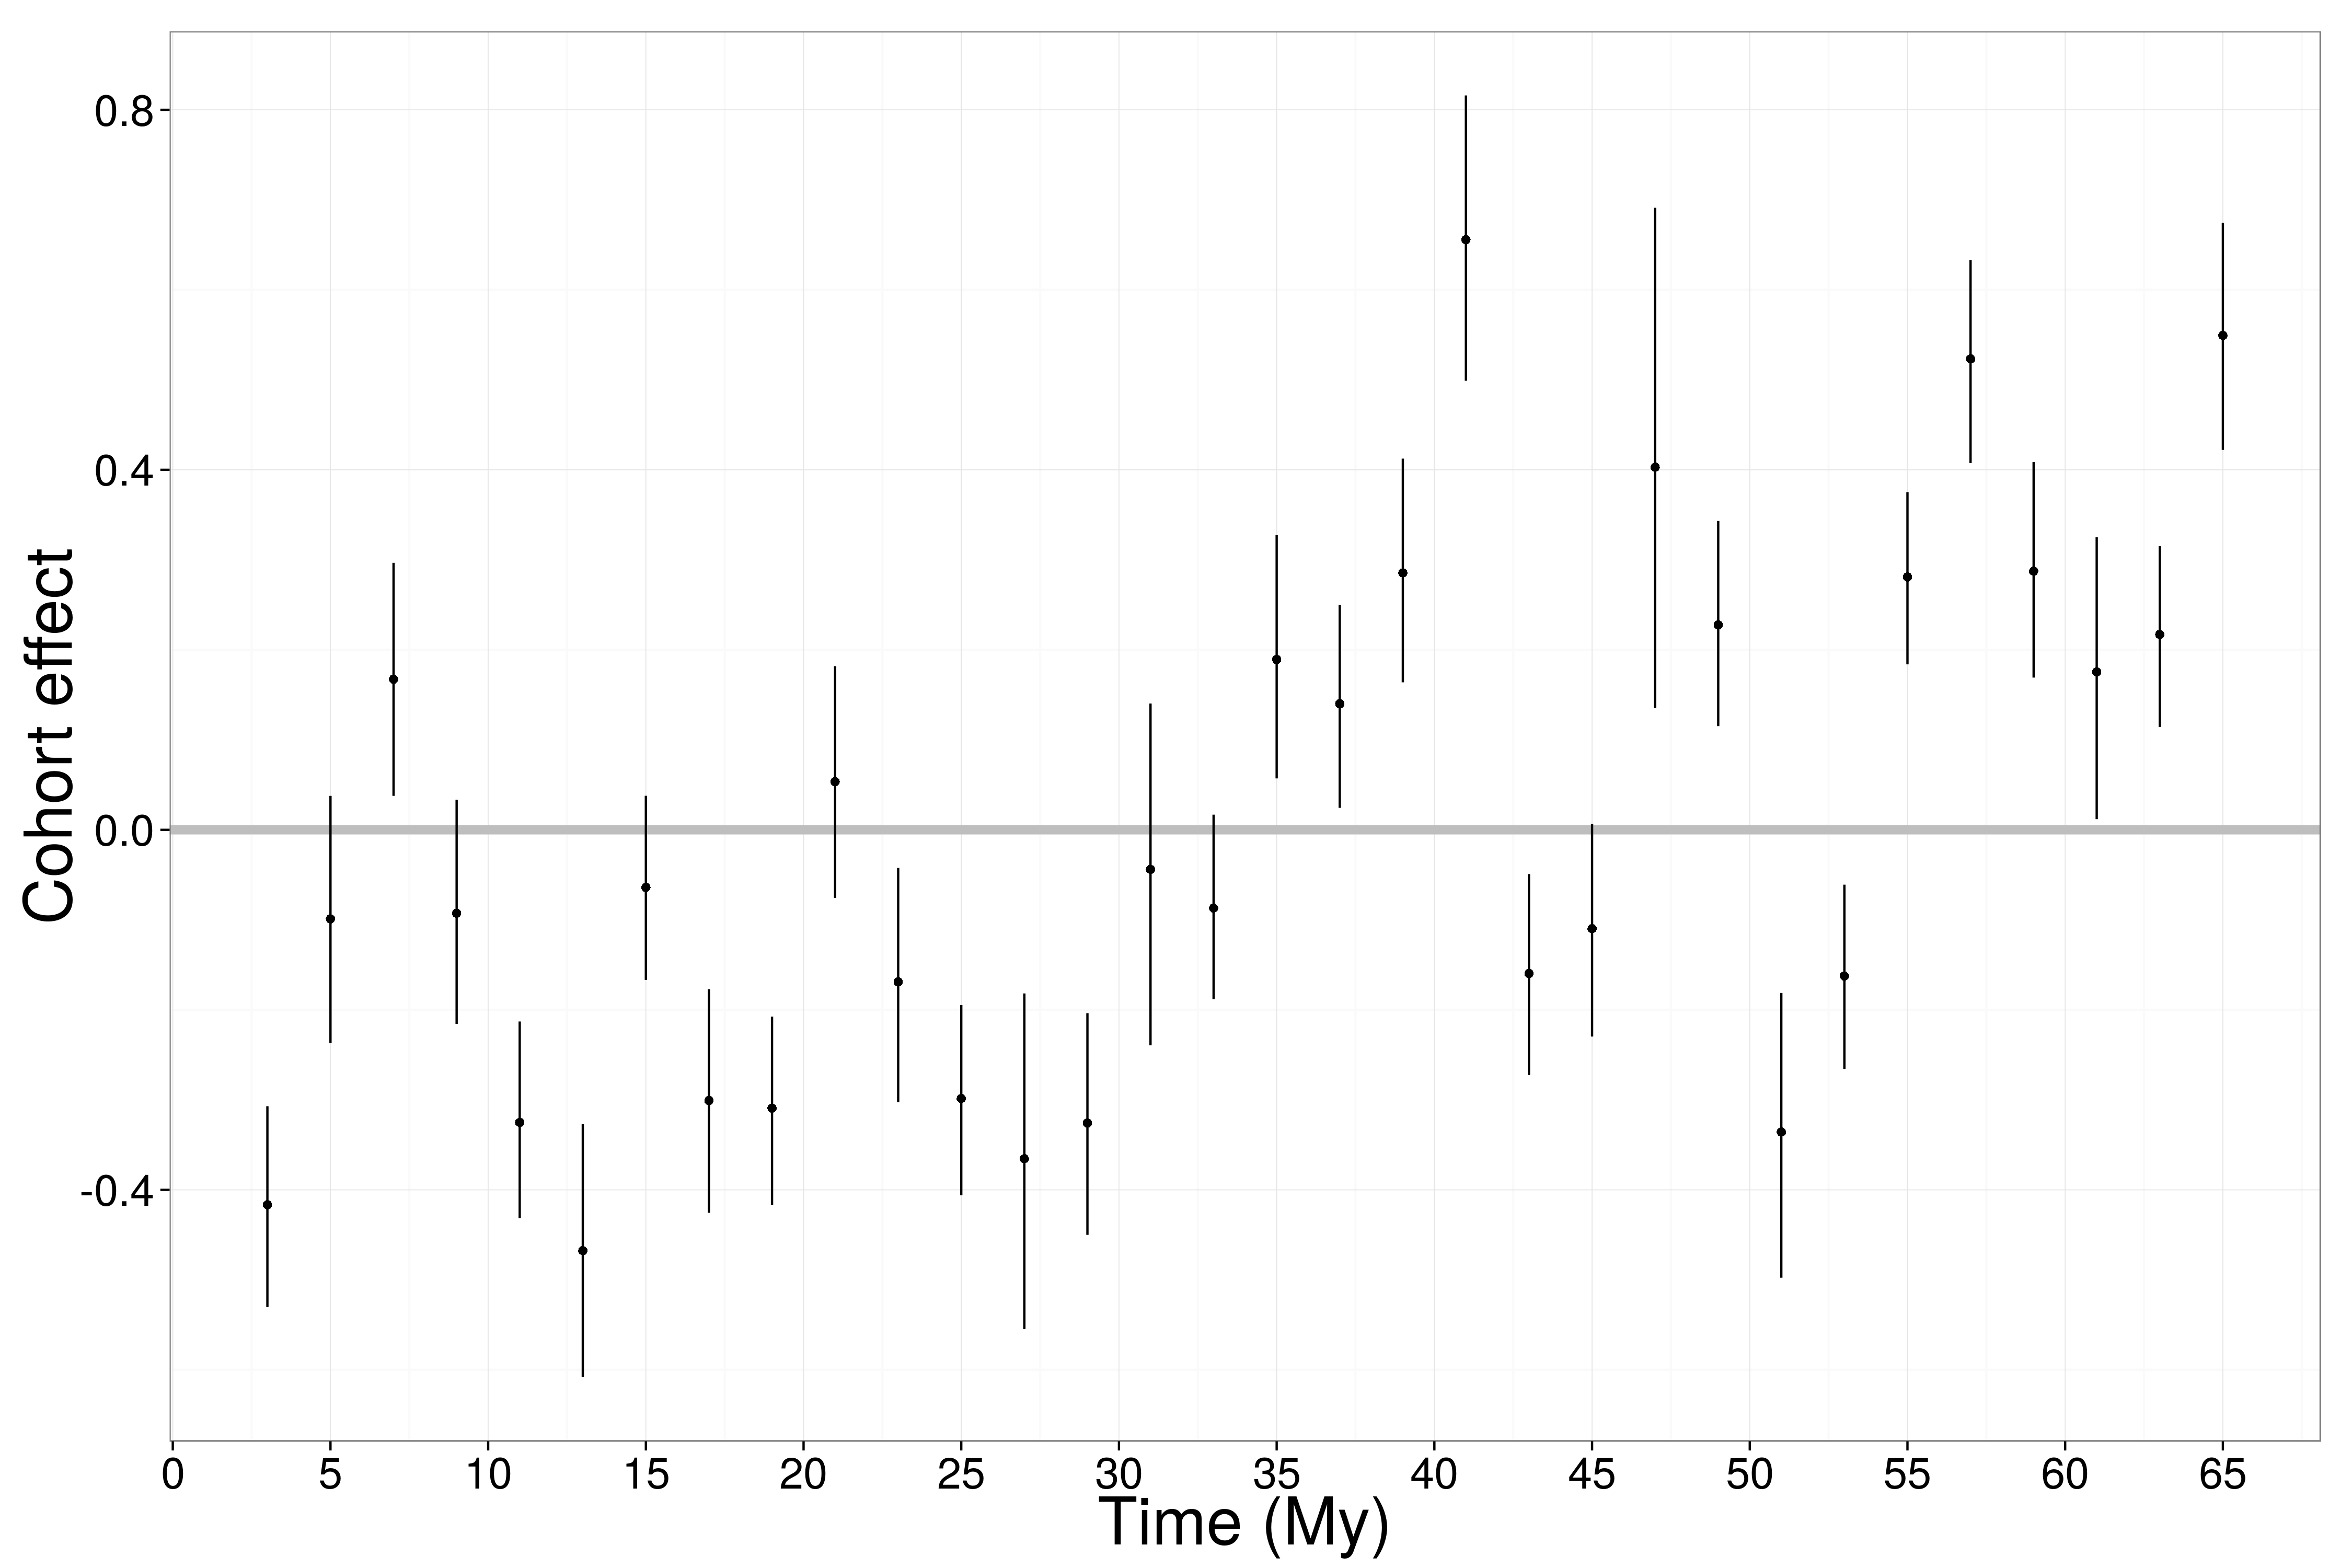
\includegraphics[height = 0.5\textheight, width = \textwidth, keepaspectratio = true]{figure/cohort_est}
  \caption{Summaries of estimated individual cohort effect posteriors. Depicted are medians and 80\% credible intervals of the estimated posterior distributions. High values correspond to shorter species durations while lower values correspond to greater species durations compared to the mean duration. Lines are placed at the middle of the 2 My origination cohorts.}
  \label{fig:eff_cohort}
\end{figure}

\begin{figure}[ht]
  \centering
  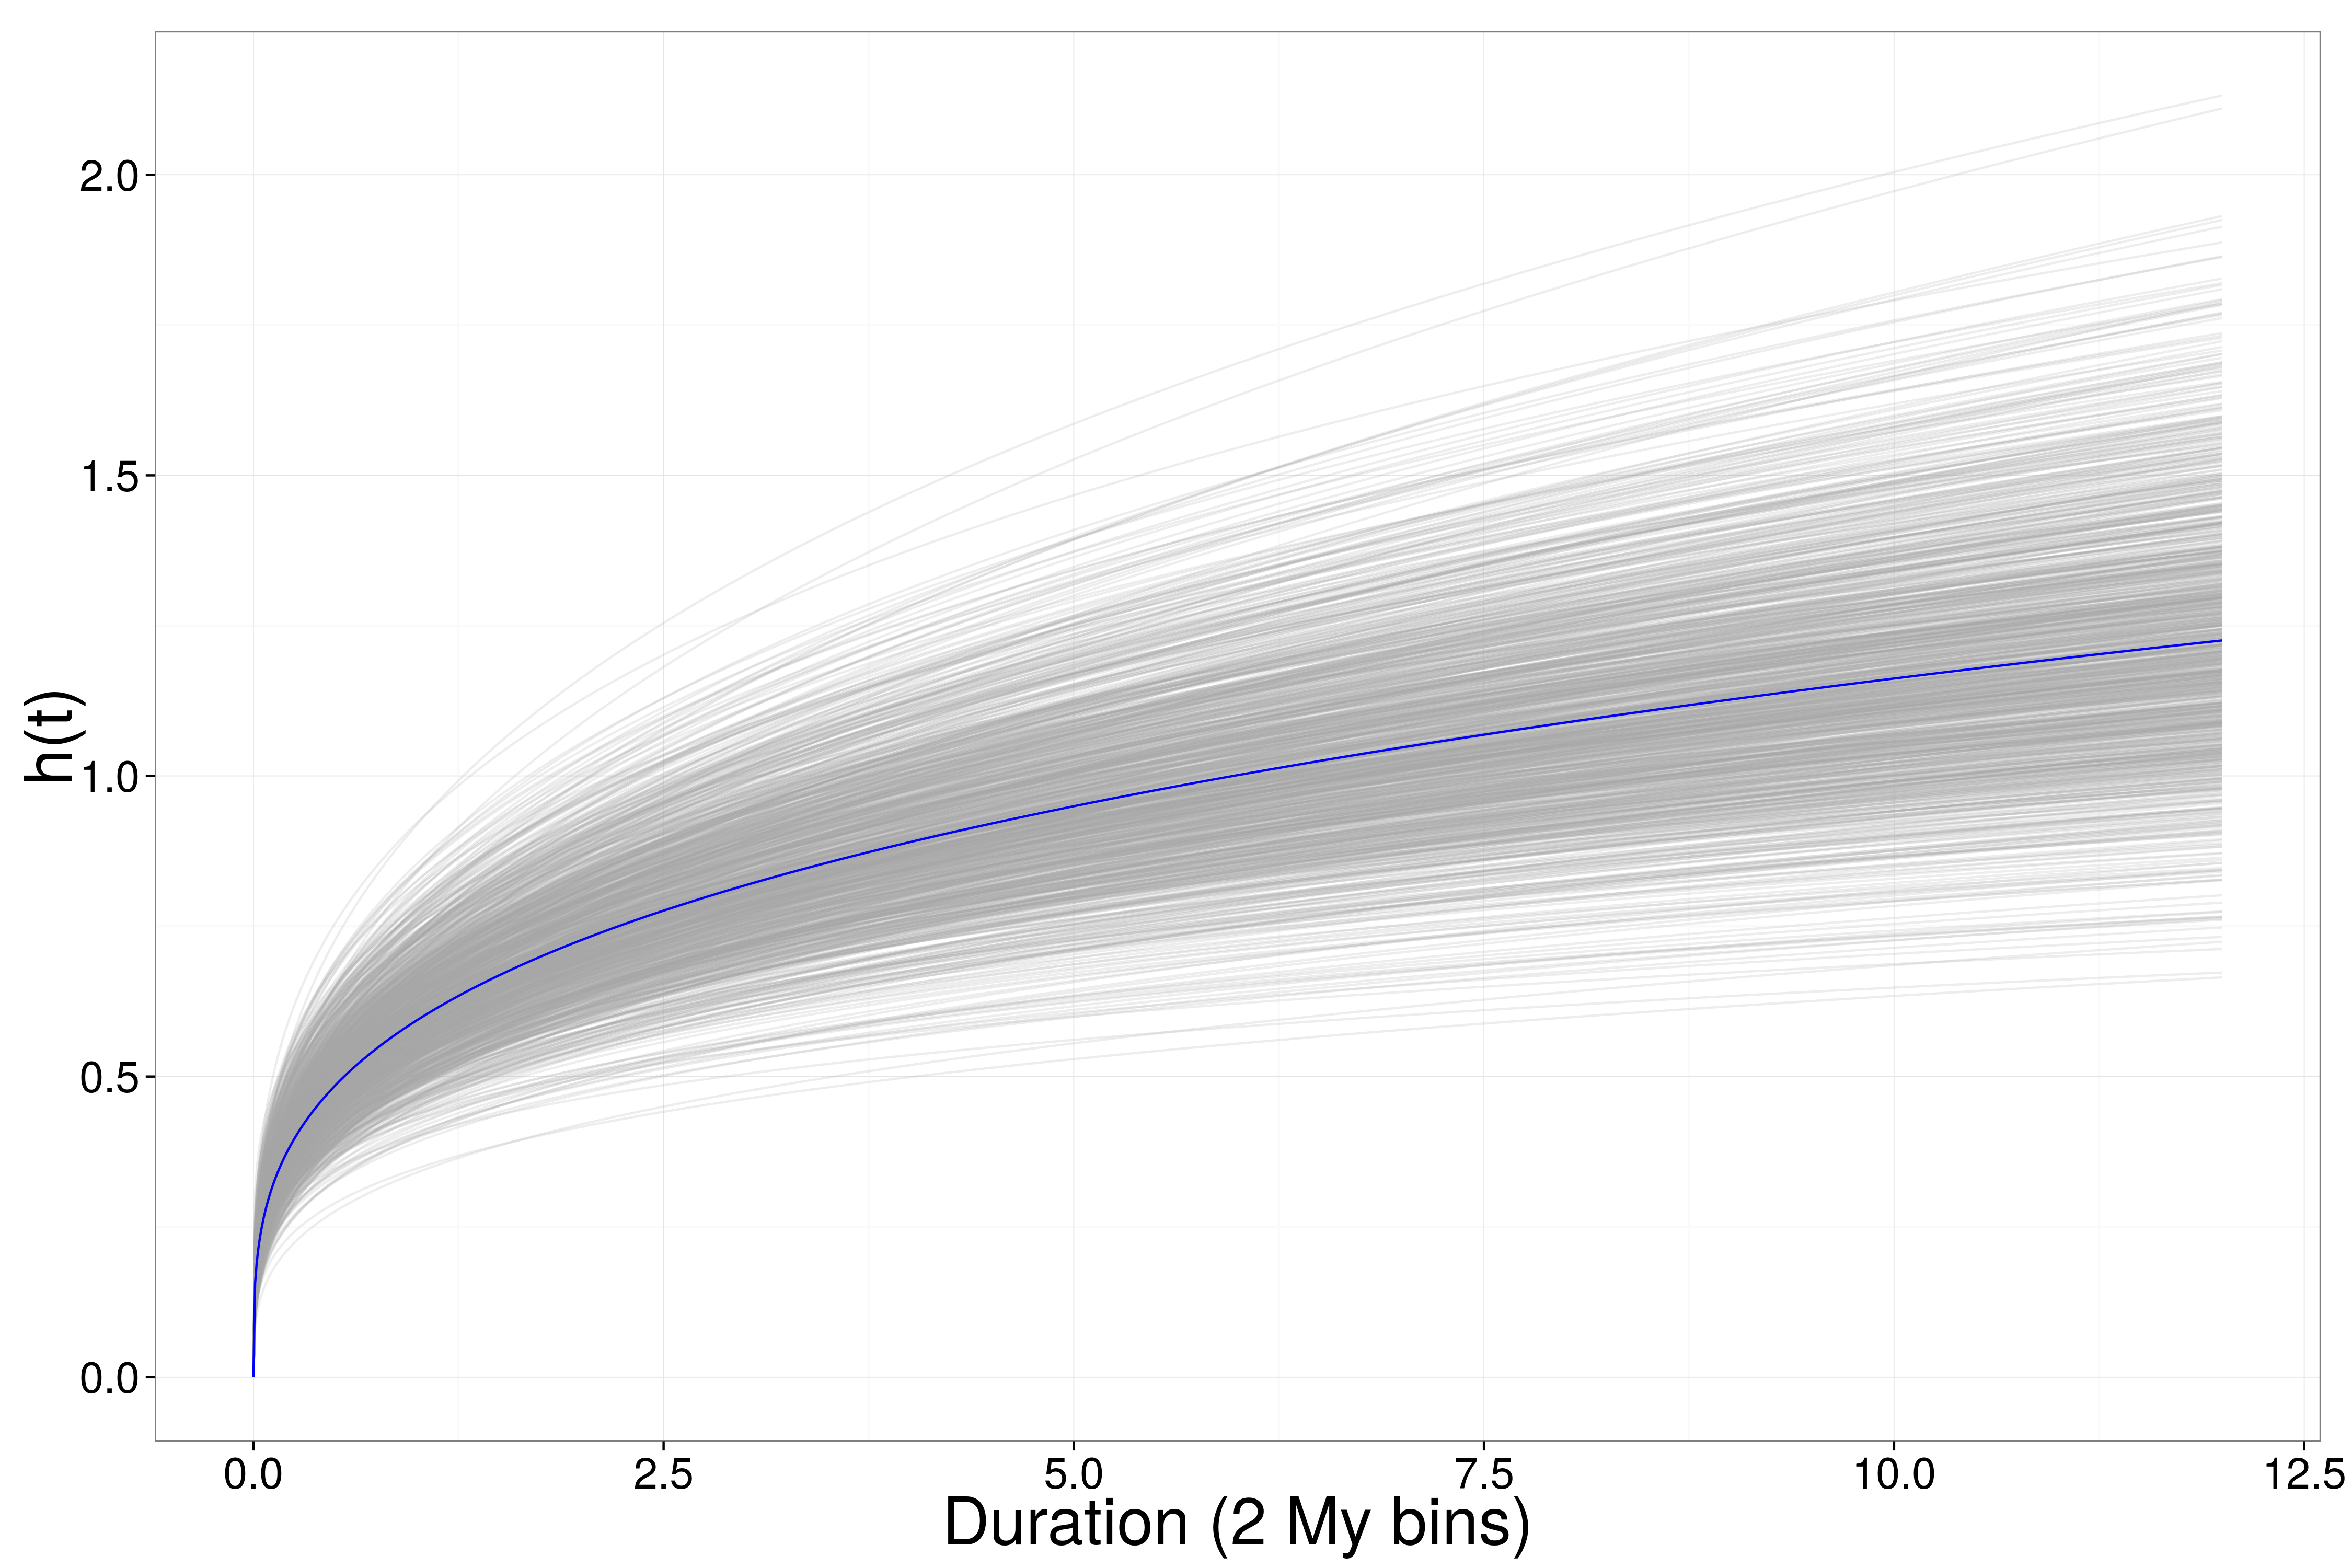
\includegraphics[height = 0.5\textheight, width = \textwidth, keepaspectratio = true]{figure/haz_est}
  \caption{100 estimates of the hazard function (\(h(t\)) for the observed species mean (grey), along with the median estimated hazard function. \(h(t)\) is an estimate of the number of extinctions that occur given an amount of time, \(t\). Hazard functions were estimated from random draws from the estimated posterior distributions and evaluated with all covariate information set to 0, which corresponds to the expected duration of the mean species.}
  \label{fig:haz}
\end{figure}

\begin{figure}[ht]
  \centering
  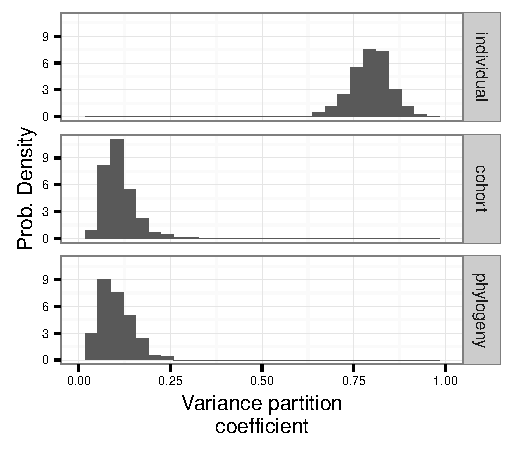
\includegraphics[height = 0.5\textheight, width = \textwidth, keepaspectratio = true]{figure/variance_est}
  \caption{Estimates of the variance partitioning coefficients for the three different sources of variance: species, cohort, and phylogeny. Higher values correspond to greater contribution to total unexplained variance. Each of the estimates is a distribution of 1000 approximating simulations due to the model's non-normality.}
  \label{fig:vpc}
\end{figure}




\end{document}
